\section{Introduction}\label{sec:introduction}
\subsection{Intent and reader prerequisites}
This manual intends to give the reader a quick introduction to the \solvername\ framework, so (s)he will be able set up and solve optimization problems. It will focus on the practical aspects rather than the theory behind the concepts used in the solver algorithm. Therefore, the reader should at least be acquainted with the following topics within the field of optimization:
\begin{itemize}
\item
Mathematical formulation of mixed-integer nonlinear programming (MINLP) optimization problems.
\item
Convexity, and the importance of convexity within optimization. A good introduction to this topic can be found in chapters 2-4 of Boyd and Vandenberghe's \emph{Convex Optimization} ~\cite{Boyd:2004:CO:993483}.
\item
Interior-point algorithms. Ipopt is an interior-point algorithm, and it is the default solver for local optimization problems in \solvername. Good introductions on interior-point algorithms are found in chapter 11 of \emph{Convex Optimization} ~\cite{Boyd:2004:CO:993483} and chapters 14 and 19 of Nocedal and Wright's \emph{Numerical Optimization} ~\cite{Nocedal99}.
\item
Branch-and-Bound algorithms. An introduction can be found in e.g.  ~\cite{clausen1999branch}.
\end{itemize}
{\color{red} TODO: Describe \solvername!!!!}
\subsection{Types of problems solved}
\solvername\ is a framework for solving general mixed-integer nonlinear programs (MINLPs) on the form
\begin{subequations} \label{eqn:minlp}
\begin{align}
\minimize f(x) &= c^{\top} x, \label{eqn:minlp_objective} \\
\subto c_i^L &\leq c_i(x) \leq c_i^U,\ \ \ i = \lbrace 1, \dots, m \rbrace \label{eqn:minlp_constraints} \\
x^L &\leq x \leq x^U \label{eqn:minlp_varbounds},
\end{align}
\end{subequations}
where $x = \begin{bmatrix} x_{\mathrm{c}}^{\top} & x_{\mathrm{i}}^{\top} \end{bmatrix}^{\top}$. $x_{\mathrm{c}} \in \mathbb{R}^{n_{\mathrm{c}}}$ is a vector of continuous optimization variables and $x_{\mathrm{i}} \in \mathbb{Z}^{n_{\mathrm{i}}}$ is a vector of integer optimization variables. The total number of optimization variables is $n = n_{\mathrm{c}} + n_{\mathrm{i}}$. The presence of integer variables and nonlinear constraints makes this problem a MINLP.
\begin{itemize}
\item
Equation (\ref{eqn:minlp_objective}) shows the objective function $f: \mathbb{R}^{n_{\mathrm{c}}} \times \mathbb{Z}^{n_{\mathrm{i}}} \mapsto \mathbb{R}$, which is assumed to be linear in the optimization variables. This does not lead to any loss of generality, since any optimization problem can be written this way by converting it to its epigraph form (see section \ref{sec:epigraph}). $c \in \mathbb{R}^n$ is a vector of constants.
\item
Equation (\ref{eqn:minlp_constraints}) shows the constraints of the MINLP. Each $c_i : \mathbb{R}^{n_{\mathrm{c}}} \times \mathbb{Z}^{n_{\mathrm{i}}} \mapsto \mathbb{R}$ is a constraint function, $c_i^L \in (\mathbb{R} \cup \lbrace -\infty \rbrace)$ is the lower bound for the constraint function and $c_i^U \in (\mathbb{R} \cup \lbrace \infty \rbrace)$ is the upper bound for the constraint function. An equality constraint is specified by setting $c_i^L = c_i^U = c_i(x)$. The number of constraints is $m$. No particular assumptions are made about the constraint functions; they can be linear or nonlinear, convex or nonconvex. However, to ensure predictable solver behaviour, they should be twice continuously differentiable.
\item
Equation (\ref{eqn:minlp_varbounds}) shows the domain bounds of each variable. $x^L \in (\mathbb{R} \cup \lbrace -\infty \rbrace )^n$ is a vector of lower bounds and $x^U \in (\mathbb{R}  \cup \lbrace \infty \rbrace )^n$ is a vector of upper bounds. Even though these constraints could be included in (\ref{eqn:minlp_constraints}),  they are stated explicitly here for the sake of simplicity.
\end{itemize}

\subsection{Supported constraint classes}
Even though any constraint can be implemented in \solvername, a few common classes of constraints have been added to the framework for simple implementation in the MINLP. The variables used in these constraints can be any of the optimization variables, continuous and/or integer. Some of the constraints specify relationships between a subset of the optimization variables. In these cases we will use the notation  $\tilde{x} \in \mathbb{R}^q \times \mathbb{Z}^r, q\leq n_{\mathrm{c}}, r \leq n_{\mathrm{i}}$ for a subset of the optimization variables. The constraint classes which are currently supported are:
\begin{itemize}
\item
Linear constraints on the form
\begin{equation}
\label{eqn:linear}
\tilde{c}^L \leq A \tilde{x} \leq \tilde{c}^U,
\end{equation}
Recall that a linear equality constraint on the form $A\tilde{x} = b$ can be specified by letting $\tilde{c}^L = \tilde{c}^U = b$. Here, $\tilde{c}^L \in (\mathbb{R} \cup \lbrace -\infty \rbrace)^{q+r}$ and $\tilde{c}^U \in ( \mathbb{R} \cup \lbrace \infty \rbrace)^{q+r}$ are vectors of upper and lower bounds corresponding to the subset of the optimization variables.
\item
Quadratic constraints on the form
\begin{equation}
\label{eqn:quadratic}
c_i^L \leq \tilde{x}^{\top} P \tilde{x} + q^{\top} \tilde{x} + r \leq c_i^U,
\end{equation}
where $P$ is a $(q+r) \times (q+r)$ matrix (not necessarily symmetric), and $q \in \mathbb{R}^{q+r}$ and $r \in \mathbb{R}$ are constant vectors.
\item
One-dimensional quadratic constraints on the form
\begin{equation}
\label{eqn:quadratic1d}
c_i^L \leq ax_0^2 + bx_0 + c - x_1 \leq c_i^U,
\end{equation}
where $a$, $b$ and $c$ are constants, and $x_0$ and $x_1$ are any two optimization variables.
\item
Bilinear constraints on the form
\begin{equation}
\label{eqn:bilinear}
c_i^L \leq ax_0 x_1 - x_2 \leq c_i^U,
\end{equation}
where $a$ is a constant, and $x_0$, $x_1$ and $x_2$ are any three optimization variables.
\item
Exponential constraints on the form
\begin{equation}
\label{eqn:exponential}
c_i^L \leq ae^{bx_0} - x_1 \leq c_i^U,
\end{equation}
where $a$ and $b$ are constants, and $x_0$ and $x_1$ are any two optimization variables.
\item
Polynomial constraints on the form
\begin{equation}
\label{eqn:polynomial}
c_i^L \leq p(\tilde{x}) \leq c_i^U.
\end{equation}
The polynomial $p(\tilde{x})$ consists of $s$ monomials, and is specified by a vector $c \in \mathbb{R}^s$ and an $s \times (q+r)$ matrix $E = \lbrace e_{i,j} \rbrace$:
\begin{equation}
\begin{array}{ccccccccccc}
p(\tilde{x}) &=& c_0 & \cdot & \tilde{x}_0^{e_{0,0}} & \cdot & \tilde{x}_1^{e_{0,1}} & \cdot & \dots & \cdot & \tilde{x}_{q+r-1}^{e_{0,q+r-1}} \\ 
&+& c_1 & \cdot & \tilde{x}_0^{e_{1,0}} & \cdot & \tilde{x}_1^{e_{1,1}} & \cdot & \dots & \cdot &  \tilde{x}_{q+r-1}^{e_{1,q+r-1}} \\
&+& \dots  \\
&+& c_{s-1} & \cdot & \tilde{x}_0^{e_{s-1,0}} & \cdot & \tilde{x}_1^{e_{s-1,1}} & \cdot & \dots & \cdot  & \tilde{x}_{q+r-1}^{e_{s-1,q+r-1}}.
\end{array}
\label{eqn:polyconstr}
\end{equation}
To clarify with an example, the polynomial defined by
\[
\tilde{x} = \begin{bmatrix} x_1 \\ x_3 \\ x_8 \end{bmatrix},\ \ \ c = \begin{bmatrix} 5 \\ 3 \\ 10 \\ 1 \end{bmatrix},\ \ \ E = \begin{bmatrix} 4 & 2 & 0  \\ 1 & 0 & 8 \\ 0 & 0 & 1 \\ 1 & 0 & 0 \end{bmatrix},
\]
with $s = 4$, would look like
\[
p(\tilde{x}) = 5 x_1^4 x_3^2 + 3 x_1 x_8^8 + 10 x_8 + x_1.
\]
\item
Sine function constraints on the form
\begin{equation}
\label{eqn:sine}
c_i^L \leq a \sin (bx_0) - x_1 \leq c_i^U,
\end{equation}
where $a$ and $b$ are constants, and $x_0$ and $x_1$ are any two optimization variables.
\end{itemize}

Constraints which do not fit into any of the classes above, can be implemented in one of two ways:
\begin{itemize}
\item
Creating a new constraint class which matches the constraint exactly.
\item
Sampling the constraint in a grid and create a B-spline approximation of the constraint (see section \ref{sec:bspline} for details).
\end{itemize}

\subsection{Mathematical background}
\label{sec:mathematicalbakground}
This section discusses a few of the mathematical concepts needed to better understand how \solvername\ works. The \emph{epigraph form} is a transformation of an optimization problem to a form with a linear objective, which we need in \solvername. \emph{Convexity} and \emph{convex relaxations} are important topics in optimization theory in general, and in Branch-and-Bound algorithms such as \solvername, good convex relaxations are essential for a global solution to be found. The \emph{B-spline} is a powerful approximation and interpolation technique that can be used in \solvername\ to approximate nonlinear functions with piecewise polynomials. Also, we can easily find good convex relaxations of B-splines, which is a very useful property. We also introduce global optimization and the Branch-and-Bound algorithm.

\subsubsection{The epigraph form} \label{sec:epigraph}
Before implementing the optimization problem in \solvername, we state the problem in its \emph{epigraph form}. This is done by taking the original minimization problem (\ref{eqn:minlp}),  introducing an additional slack variable $t$, and minimizing $t$ subject to an additional constraint which says that $t$ should be greater than or equal to the original objective $f(x)$:
\begin{subequations} \label{eqn:minlp_epiform}
\begin{align}
\minimize t, \label{eqn:minlp_epiform_objective} \\
\subto f(x) - t &\leq 0, \label{eqn:minlp_epiform_newconstr} \\
c_i^L \leq c_i(x) &\leq c_i^U,\ \ \ i = \lbrace 1, \dots, m \rbrace \label{eqn:minlp_epiform_constraints} \\
x^L \leq x &\leq x^U \label{eqn:minlp_epiform_varbounds},
\end{align}
\end{subequations}
That is, we want to find the smallest $t$ that lies on or above the graph space of $f(x)$. This is illustrated in Figure \ref{fig:epigraph}. We now have a new objective function which is linear (and convex). This conversion is always possible, meaning we can assume that we only have to deal with nonconvexity and nonlinearity in the constraints. From Figure \ref{fig:epigraph} we see that $(x^*, t^*)$ is optimal for (\ref{eqn:minlp_epiform}) if and only if $x^*$ is optimal for (\ref{eqn:minlp}) and $t = f(x)$. 
\begin{figure}[H]
\centering
\subfigure[Standard form]{
	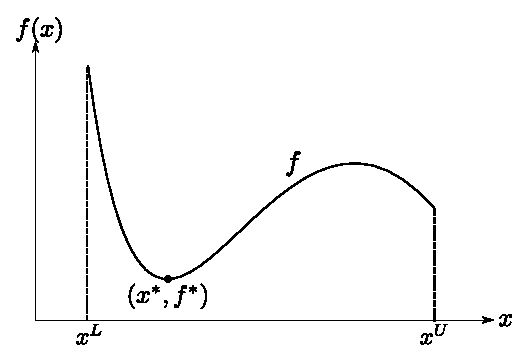
\includegraphics[scale=0.7]{figures/epigraph1.eps} 
	\label{fig:epi1}
}
\subfigure[Epigraph form. Note that  (\ref{eqn:minlp_epiform_newconstr}) constrains feasible points $(x,t)$ to lie on or above the graph space of $f(x)$, which we denote $\mathbf{epi}\ f$.]{
	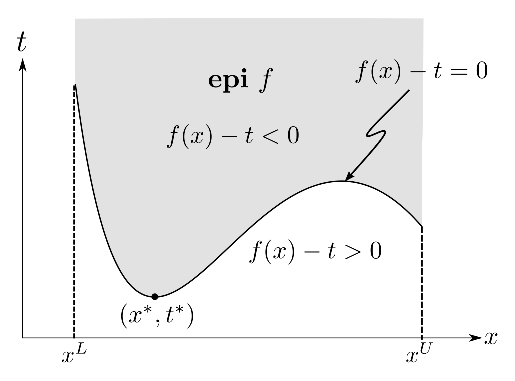
\includegraphics[scale=0.7]{figures/epigraph2.eps} 
	\label{fig:epi2}
}
\caption{Graphical representation of a standard form optimization problem and an epigraph form optimization problem.}
\label{fig:epigraph}
\end{figure}

\subsubsection{Convexity and convex relaxations}
\paragraph{Convex optimization problems.}
It is well known that a solution to an optimization problem obtained by a local solver such as Ipopt is not necessarily the global solution. However, if the optimization problem is convex, we can guarantee that the solution is the global solution. For an optimization problem to be convex, the following conditions must be satisfied:
\begin{itemize}
\item
The objective function $f(x)$ must be convex. This is always the case in (\ref{eqn:minlp_epiform}), since the objective function (\ref{eqn:minlp_epiform_objective}) is linear.
\item
The inequality constraints must be convex.
\item
The equality constraint must be linear.
\end{itemize}
\paragraph{Convex functions.} A function $f: \mathbb{R}^n \mapsto \mathbb{R}$ is \emph{convex} when the following is satisfied:
\begin{equation}
f(\alpha x_1 + \beta x_2) \leq \alpha f(x_1) + \beta f(x_2),
\label{eqn:convexitycond}
\end{equation}
for all $x_1,x_2\in \mathbb{R}^n$ and all $\alpha, \beta \in \mathbb{R}$ with $\alpha + \beta = 1,\ \alpha \geq 0,\ \beta \geq 0$. This means that a line joining two points $x_1$ and $x_2$ on $f$ will lie on or above $f$ for all choices of $x_1$ and $x_2$.
\\
\begin{figure}[H]
\centering
\subfigure[A non-convex function. The line joining $(x_1, f(x_1))$ and $(x_2, f(x_2))$ lies below the graph of $f$, violating the convexity condition (\ref{eqn:convexitycond}). This is indicated in red. The green line joining $(x_2, f(x_2))$ and $(x_3, f(x_3))$ lies above $f$, meaning $f$ is convex in this interval.] {
	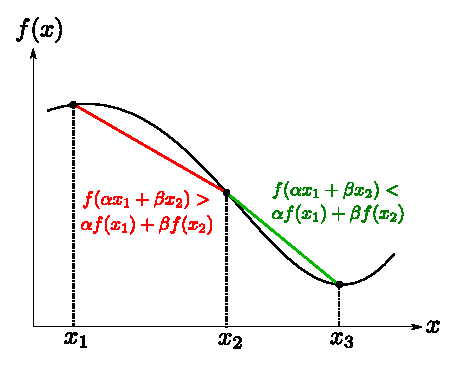
\includegraphics[scale=0.7]{figures/convex1.eps} 
	\label{fig:convex1}
}
\subfigure[A convex function. No matter where we choose to place $x_1$, $x_2$ and $x_3$, the lines joining the points lie above $f$. ]{
	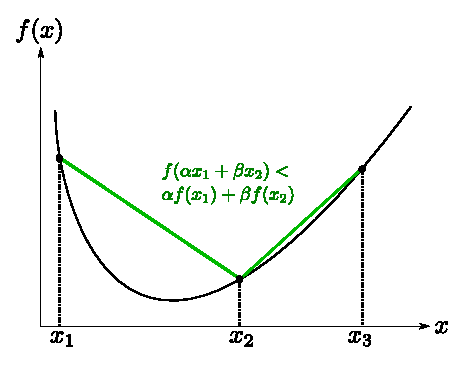
\includegraphics[scale=0.7]{figures/convex2.eps} 
	\label{fig:convex2}
}
\caption{Convex and non-convex functions.}
\label{fig:convex}
\end{figure}
Linear functions are convex, because all points on a line joining two points on the function would coincide with the function itself. Functions with positive curvature in the entire function domain (positive definite Hessian) are convex.

\paragraph{Convex sets.}
\paragraph{Convex hulls.}
\paragraph{Convex relaxations.}

\subsubsection{The B-spline} \label{sec:bspline}

\subsubsection{Global optimization and the Branch-and-Bound algorithm} \label{sec:global}

\subsection{Availability} \label{sec:availability}
\solvername\ is not publically available as of today.

\subsection{Prerequisites} \label{sec:prerequisites}
\solvername\ relies on a few open-source libraries to function. The most important of these are listed below.

\subsubsection{Ipopt} \label{sec:ipopt}
Ipopt is the default solver used in \solvername\ for solving optimization problems locally. Ipopt uses an interior point algorithm to find local solutions of (\ref{eqn:minlp}). For more information on Ipopt and installation instructions, the reader is referred to the {\color{blue} \href{https://projects.coin-or.org/Ipopt}{Ipopt home page}}. Details about the algorithm itself can be found in ~\cite{Wachter2006}.

\subsubsection{Eigen} \label{sec:eigen}
Eigen is a C++ template library for linear algebra. It includes functionality for Matlab-like matrix and vector operations, solvers and other related algorithms such as matrix decompositions. For more information on Eigen and installation instructions, the reader is referred to the {\color{blue} \href{http://eigen.tuxfamily.org/index.php?title=Main_Page}{Eigen web site}} ~\cite{eigenweb}.